\chapter{\IfLanguageName{dutch}{Stand van zaken}{State of the art}}%
\label{ch:stand-van-zaken}

% Tip: Begin elk hoofdstuk met een paragraaf inleiding die beschrijft hoe
% dit hoofdstuk past binnen het geheel van de bachelorproef. Geef in het
% bijzonder aan wat de link is met het vorige en volgende hoofdstuk.

% Pas na deze inleidende paragraaf komt de eerste sectiehoofding.

% Dit hoofdstuk bevat je literatuurstudie. De inhoud gaat verder op de inleiding, maar zal het onderwerp van de bachelorproef *diepgaand* uitspitten. De bedoeling is dat de lezer na lezing van dit hoofdstuk helemaal op de hoogte is van de huidige stand van zaken (state-of-the-art) in het onderzoeksdomein. Iemand die niet vertrouwd is met het onderwerp, weet nu voldoende om de rest van het verhaal te kunnen volgen, zonder dat die er nog andere informatie moet over opzoeken \autocite{Pollefliet2011}.

% Je verwijst bij elke bewering die je doet, vakterm die je introduceert, enz.\ naar je bronnen. In \LaTeX{} kan dat met het commando \texttt{$\backslash${textcite\{\}}} of \texttt{$\backslash${autocite\{\}}}. Als argument van het commando geef je de ``sleutel'' van een ``record'' in een bibliografische databank in het Bib\LaTeX{}-formaat (een tekstbestand). Als je expliciet naar de auteur verwijst in de zin (narratieve referentie), gebruik je \texttt{$\backslash${}textcite\{\}}. Soms is de auteursnaam niet expliciet een onderdeel van de zin, dan gebruik je \texttt{$\backslash${}autocite\{\}} (referentie tussen haakjes). Dit gebruik je bv.~bij een citaat, of om in het bijschrift van een overgenomen afbeelding, broncode, tabel, enz. te verwijzen naar de bron. In de volgende paragraaf een voorbeeld van elk.

% \textcite{Knuth1998} schreef een van de standaardwerken over sorteer- en zoekalgoritmen. Experten zijn het erover eens dat cloud computing een interessante opportuniteit vormen, zowel voor gebruikers als voor dienstverleners op vlak van informatietechnologie~\autocite{Creeger2009}.

% Let er ook op: het \texttt{cite}-commando voor de punt, dus binnen de zin. Je verwijst meteen naar een bron in de eerste zin die erop gebaseerd is, dus niet pas op het einde van een paragraaf.


% \begin{figure}
%   \centering
%   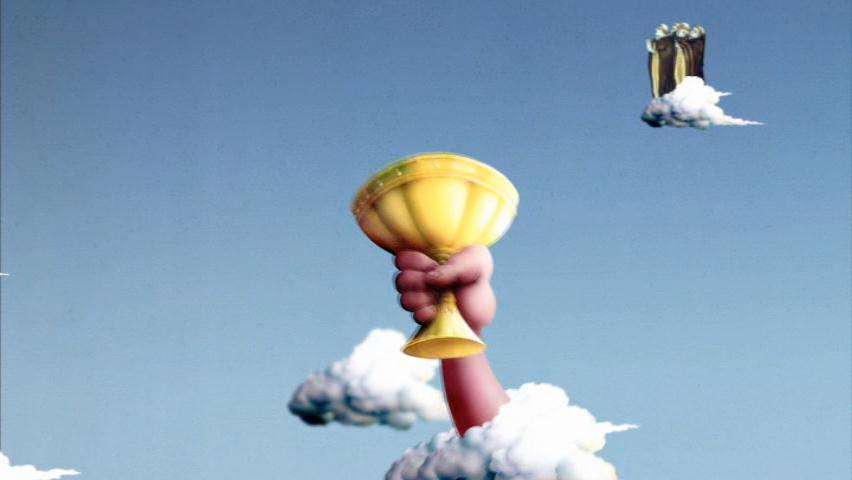
\includegraphics[width=0.8\textwidth]{grail.jpg}
%   \caption[Voorbeeld figuur.]{\label{fig:grail}Voorbeeld van invoegen van een figuur. Zorg altijd voor een uitgebreid bijschrift dat de figuur volledig beschrijft zonder in de tekst te moeten gaan zoeken. Vergeet ook je bronvermelding niet!}
% \end{figure}

% \begin{listing}
%   \begin{minted}{python}
%     import pandas as pd
%     import seaborn as sns

%     penguins = sns.load_dataset('penguins')
%     sns.relplot(data=penguins, x="flipper_length_mm", y="bill_length_mm", hue="species")
%   \end{minted}
%   \caption[Voorbeeld codefragment]{Voorbeeld van het invoegen van een codefragment.}
% \end{listing}

% \begin{table}
%   \centering
%   \begin{tabular}{lcr}
%     \toprule
%     \textbf{Kolom 1} & \textbf{Kolom 2} & \textbf{Kolom 3} \\
%     $\alpha$         & $\beta$          & $\gamma$         \\
%     \midrule
%     A                & 10.230           & a                \\
%     B                & 45.678           & b                \\
%     C                & 99.987           & c                \\
%     \bottomrule
%   \end{tabular}
%   \caption[Voorbeeld tabel]{\label{tab:example}Voorbeeld van een tabel.}
% \end{table}

Geautomatiseerde dataverzameling en -analyse spelen een steeds grotere rol in de professionele sportwereld, waar nauwkeurige statistieken noodzakelijk zijn voor prestatieverbetering en strategische besluitvorming. In de sport, in het bijzonder in volleybal, zorgt automatisering van statistieken verzameling ervoor dat spelers en coaches beter inzicht krijgen in prestaties, waardoor training en wedstrijdvoorbereiding doelgerichter kunnen worden aangepakt.
\subsection{Belang van statistieken in de sportwereld}
Vooral technologieën zoals AI, computer vision en machine learning bieden nieuwe mogelijkheden om spelmomenten en spelersbewegingen nauwkeurig vast te leggen en te analyseren. De spelers- en matchstatistieken \autocite{Wahyuti2023} zijn van uiterst belang. Ze bieden niet alleen inzichten in de puntenregistratie van het team, maar ook in de tactische en technische aspecten van het spel. Volgens de studie is het belangrijk om een uitgebreid digitaal puntenregistratie bij te houden. Dit om fouten en verlies van gegevens te minimaliseren. Dit komt echter vaak voor bij handmatige invoer. Uit onderzoek \autocite{Harabagiu2023} blijkt dat door het gebruik van door gebruik van de statistische software Data Volley de efficiënte van een team met 6\% stijgt. De software identificeert de tekortkomingen en hierdoor kunnen individuele trainingsprogramma's opgesteld worden voor elke speler. Volgens \textcite{Ruiye2024} zijn de nauwkeurigheid en efficiëntie van de videoanalyse zeer belangrijk. Een innovatief videoanalysemodel gebaseerd op Bi-directional Long Short-Term Memory (BiLSTM) en aandachtsmechanismen behaalt een herkenningsnauwkeurigheid van meer dan 90%.

Natuurlijk zijn er andere invloeden op de statistieken dan alleen de spelersprestaties \autocite{LopezSerrano2022}. Zo spelen volgens verschillende coaches het niveau van de tegenstander, het moment in een set, het scoreverschil, resultaat van de vorige set en het de competitieve druk een zeer grote in de analyse. Trainers pleiten ervoor dat er een geïntegreerde benadering is voor deze variabelen. Hierdoor wordt rekening gehouden met de specifieke omstandigheden van elke wedstrijd. Deze gegevens mogen niet geïsoleerd worden bekeken, maar juist in samenhang geanalyseerd. Bij verder onderzoek is het van essentieel belang dat coaches worden betrokken bij de ontwikkeling hiervan.
% Bestaande AI-oplossingen voor sportstatistieken

% Gebruik van sensors en camera's voor dataverzameling
\subsection{Gebruik van sensors en camera's voor dataverzameling}
Uit onderzoek van Xu Sun \textcite{Sun2021} blijkt dat door de vooruitgang in elektronische en sensortechnologieën is het mogelijk geworden om menselijke bewegingen en spelmomenten nauwkeurig vast te leggen. In de sportwereld zijn sensoren en camera's steeds vaker te vinden op en naast het veld. Deze technologieën maken het mogelijk om realtime data te verzamelen over spelersposities, balbewegingen en spelsituaties door middel van sensoren aan de gewrichten van spelers te bevestigen. Door deze data te analyseren met behulp van AI-algoritmen kunnen coaches en analisten waardevolle inzichten verkrijgen in de prestaties en strategieën.

\textcite{Liang2023} concludeerden dat traditionele videoanalysemethode vaak te beperkt zijn voor de variabele omstandigheden zoals verlichting en achtergrond tijdens het spel. Skeletdata biedt hier een oplossing voor door de bewegingen van spelers te vereenvoudigen tot een netwerk van verbonden gewrichten. De complexiteit van de visuele gegevens vermindert hierdoor. De methode zou nog een extra assistentie kunnen bieden aan de coaches en spelers.
